\documentclass{beamer}

\usepackage[utf8]{inputenc}
\usetheme{default}

\usepackage{listings}
\lstset{
basicstyle=\small\ttfamily,
columns=flexible,
breaklines=true
}

\usepackage{epstopdf}
\usepackage{multicol}

\makeatletter
\DeclareMathSizes{\f@size}{10}{7}{7}
\makeatother

\title[66.20/86.37]{U.B.A. - Facultad de Ingeniería\\\vspace{0.25cm} 66.20/86.37 Organización de Computadoras
\\Arquitecturas}
\author{Práctica}
\date{1$^{er}$ cuatrimestre 2020}


\begin{document}
\begin{frame}
\titlepage % Print the title page as the first frame
\end{frame}

\begin{frame}
\frametitle{Clasificación de ISAs}
\begin{center}
 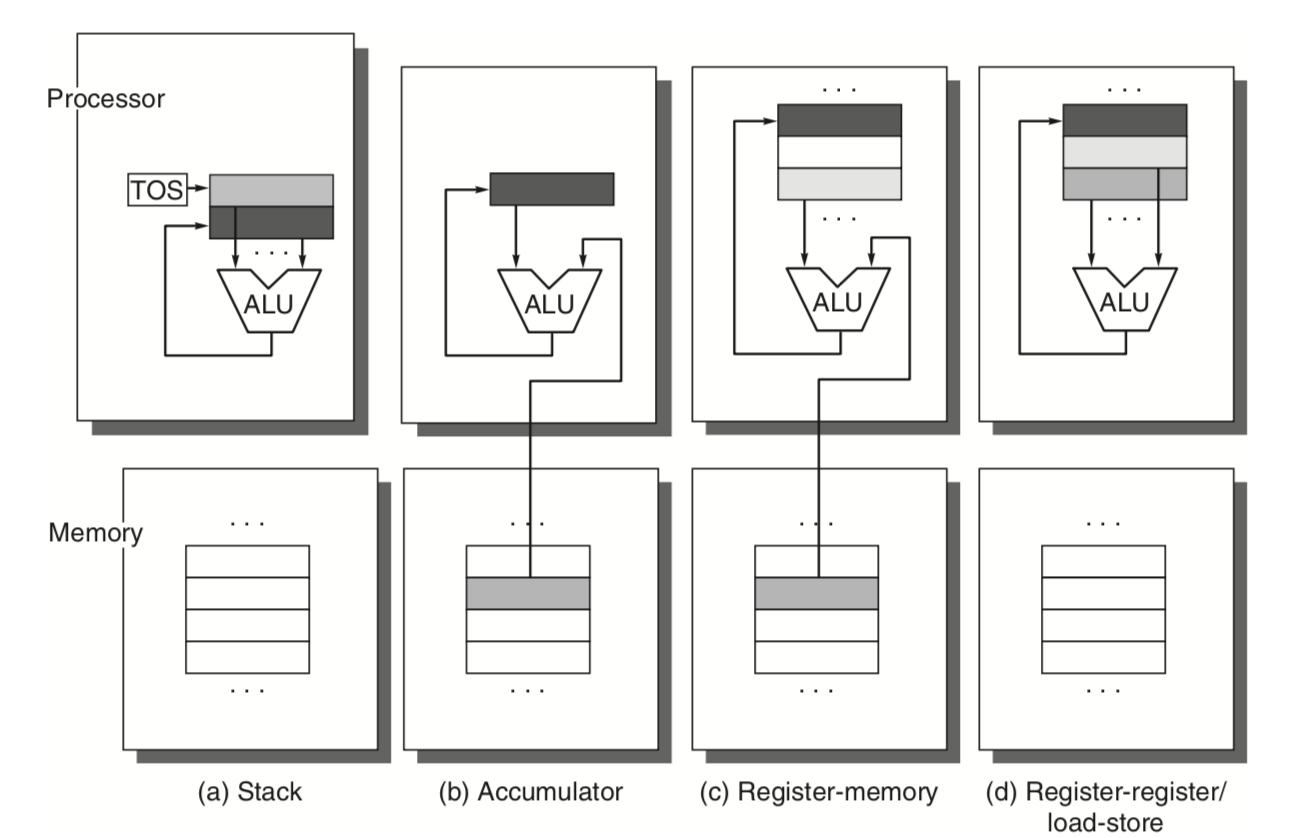
\includegraphics[scale=.45,keepaspectratio=true]{ISA.png}
\end{center}
\end{frame}

\begin{frame}
 \frametitle{Clasificación de ISAs}
 \begin{itemize}
  \item Modelo de pila: 
Los operandos están implícitamente en el tope del stack y el hardware debe evaluar la expresión en un solo orden y cargar un operando múltiples veces.
\item Modelo de acumulador: 
En una arquitectura de acumulador un operando está implícito en el acumulador.
\item Modelo de registros de propósito general: 
Aquí se tienen únicamente operandos explícitos, ya sea que estén ubicados en registros o en memoria.
\item Modelo de carga y almacenamiento: 
En este tipo de arquitectura, la memoria solo puede ser accedida a través de instrucciones de carga y almacenamiento (load/store). 
 \end{itemize}
\end{frame}


\begin{frame}
 \frametitle{Tipo de instrucciones en MIPS}
 \begin{itemize}
  \item Load / Store: únicas que acceden a memoria.
  \item Computational: realizadas en la ALU.
  \item Jump / Branch: saltos incondicionales y condicionales.
  \item Miscelaneas: Serialización de instrucciones, Excepciones (syscall), Moves condicionales, Prefetch, NOPs.
  \item Coprocessors y FPU.
 \end{itemize}
\end{frame}

\begin{frame}
 \frametitle{Ejercicio 2.1 CAAQA 3ed}
 
For the following assume that values A, B, C, D and E reside in memory. Also assume that instruction operation codes are represented in 8 bits, memory addresses are 64 bits, and register addresses are 6 bits.

\begin{enumerate}[a]
 \item For each instruction set architecture shown in Figure 2.2, how many addresses, or names, appear in each instruction for the code to compute C = A + B and what is the total code size?

 \item Some of the instruction set architectures in figure 2.2 destroy operands in the course of computation. This loss of data values from processor internal storage has performance consequences. For each architecure in Figure 2.2 write the code sequence to compute C = A + B followed by D = A - E. In your code, mark each operand that is destroyed during execution and mark each "overhead" instruction that is included just to overcome this number of overhead instructions, and the number of overhead data bytes for each of your code sequences?
\end{enumerate}
\end{frame}

\begin{frame}
 \frametitle{Ejercicio 2.2 CAAQA 3ed}
 Some operations on two operands (substraction, for example) are not commutative. What are the advanges and disadvantages of the stack, accumulator, and load-store architectures when executing noncummutative operations?
\end{frame}


\begin{frame}
 \frametitle{Endianess}
Todo el conjunto de instrucciones es direccionado por bytes y se provee acceso por bytes (8 bits), mitad de palabra (half words) (16 bits), por palabra (words) (32 bits).

\bigskip

Hay dos convenciones para ordenar los bytes en un objeto. \textbf{Little Endian} y \textbf{Big Endian}.
 \end{frame}
 
\begin{frame}
 \frametitle{Endianess}

El orden \textbf{Little Endian} coloca el byte cuya dirección "x . . . x000” en la posición menos significativa. Los bytes entonces son numerados:

  \begin{center}
 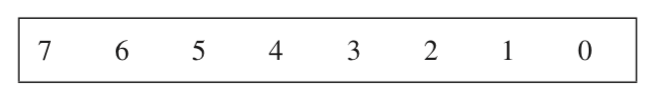
\includegraphics[scale=.7,keepaspectratio=true]{little_endian.png}
\end{center}


El orden \textbf{Big Endian} coloca el byte cuya dirección es “x . . . x000”  en la posición más significativa. Los bytes entonces son numerados:

\begin{center}
 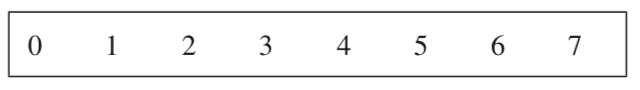
\includegraphics[scale=.7,keepaspectratio=true]{big_endian.png}
\end{center}

 \end{frame}


\begin{frame}
 \frametitle{Alineación}
 En varias computadoras, los accesos a objetos más grandes que un byte deben estar alineados.
 \begin{itemize}
  \item Un objeto de tamaño s bytes en la dirección de bytes A está alineado si
    A mod s = 0.
  \item Esto se fuerza en muchas arquitecturas porque el hardware accede a
    memoria típicamente alineado a múltiplos de word o double-word.
 \end{itemize}
\bigskip
 ¿Qué puede ocurrir a nivel de accesos a memoria si se accede a datos no alineados y la arquitectura lo permite?
    
\end{frame}

\begin{frame}
 \frametitle{Modos de direccionamiento}
Se presentan varios modos de direccionamiento: 
\begin{multicols}{2}
\begin{itemize}
 \item Register
 \item Immediate
 \item Displacement
 \item Register indirect
 \item Indexed
 \item Direct or Absolute
 \item Memory indirect
 \item Autoincrement
 \item Autodecrement
 \item Scaled
 \end{itemize}
\end{multicols}

MIPS implementa 2 modos de direccionamiento: Immediate y Displacement, ambos con immediate de 16 bits.
    
Usando el registro 0 se consigue Absolute, y con displacement 0 se consigue Register indirect.
\end{frame}

\begin{frame}[fragile]
\frametitle{Modos de direccionamiento}

\begin{lstlisting}
    Immediate:		add	$t1, $t2, 10	
    Displacement:	lw	$t1, 30($t2)
    Absolute:		sb	$t1, 40($0)
    Indirect:		sw	$t1, 0($t2)
\end{lstlisting}
\end{frame}

\begin{frame}
 \frametitle{Ejercicio 2.3 CAAQA 3ed}
 The value represented by the hexadecimal number 434F 4D50 5554 4552 is to be stored in an aligned 64-bit double word.
 
 \begin{enumerate}[a.]
  \item Using the physical arrangement of the first row in Figure 2.5, write the value to be stored using Big Endian byte order. Next, interpret each byte as an ASCII character and below each byte write the correspondig character, forming the character string as it would be stored in Big Endian order.
  
  \item Using the same physical arrangement as in part (a.), write the value to be stored using the Little Endian byte order and below each byte write the corresponding ASCII character.
 \end{enumerate}

\end{frame}

\begin{frame}
 \frametitle{Encoding MIPS} 
 Hay 3 formatos de encoding posibles en MIPS
 \begin{itemize}
  \item I-type (Immediate)
  \item R-type (Register)
  \item J-type (Jump)
 \end{itemize}
\end{frame}

\begin{frame}
 \frametitle{Encoding MIPS} 
 
 \begin{center}
 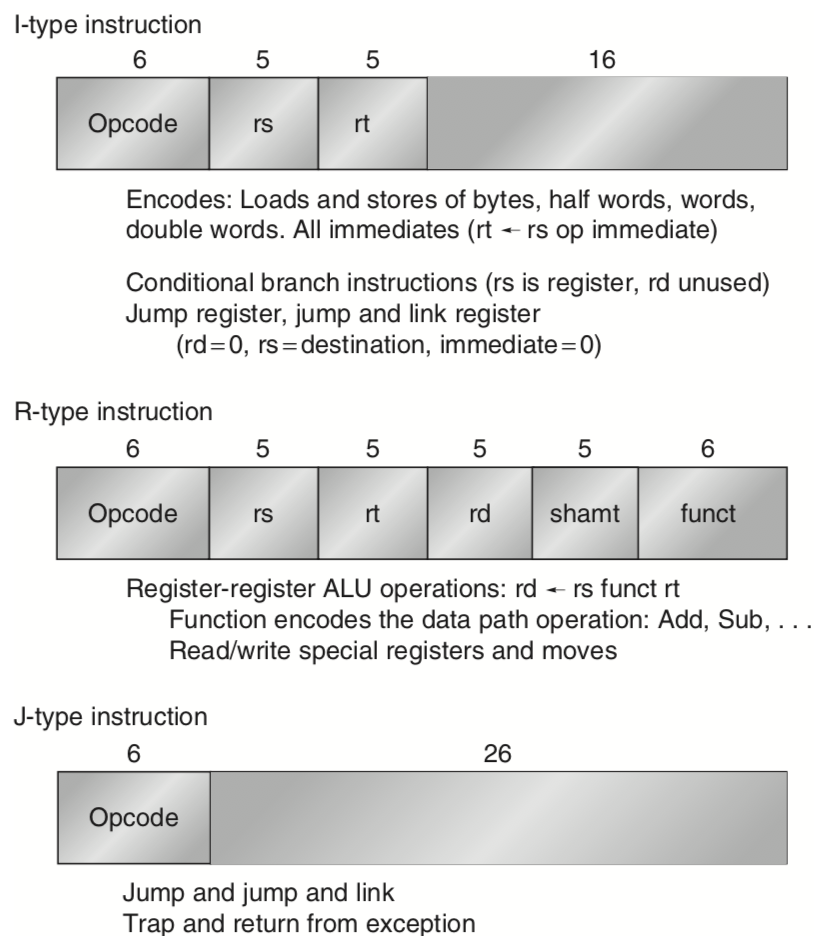
\includegraphics[scale=.4,keepaspectratio=true]{tipos_instruccion.png}
\end{center}
 \end{frame}


\begin{frame}
 \frametitle{Encoding MIPS} 

 Viendo el detalle de las intrucciones J-type vemos que hay un offset de 26 bits left-shifted 2 bits, para formar los 28 lsb de la direccion destino del salto (las regiones de salto están alineadas a 256MB, y la región está determinada por los 4 msb de PC).
 
 \bigskip

 ¿Por qué se puede (y conviene) tomar los 26 bits como desplazados a la izquierda 2 bits?
\end{frame}

\begin{frame}[fragile]
 \frametitle{Ejercicio 2.6 CAAQA 3ed}
 Several reserchers have suggested that adding a register-memory addressing mode to a load store machine be useful. The idea is to replace sequences of
 
\begin{lstlisting}
 LOAD   R1, 0(Rb)
 ADD    R2, R2, R1
\end{lstlisting}

by

\begin{lstlisting}
 ADD    R2, 0(Rb)
\end{lstlisting}

Assume the new instruction will cause the clock cycle to increase by 5\%. Use the instruction frequencies for the gcc benchmark on the load-store machine from figure 2.32. The new instruction affects only the clock cycle and not the CPI.
\end{frame}
\begin{frame}
 \frametitle{Ejercicio 2.6 CAAQA 3ed}
\begin{enumerate}[a.]
 \item What percentage of the loads must be eliminated for the machine with the new instruction to have at least the same performance?
 
 \item Show a situation in a multiple instruction sequence where a load of R1 followed immediately by a use of R1 (with some type of opcode) could not be replaced by a single instruction of the form proposed, assuming that the same opcode exists.
\end{enumerate}
\end{frame}

\begin{frame}
 \frametitle{Ejercicio 2.11 CAAQA 3ed}
 Compute the effective CPI for MIPS using Figure 2.32. Suppose we have made the following measurements of average CPI for instructions:
 
 Assume that 60\% of the conditional branches are taken and that all instruction in the ``other'' category of Figure 2.32 are ALU instructions. Average the instruction fracuencies of gap and gcc to obtain the instruction mix.
\end{frame}

\begin{frame}[fragile]
 \frametitle{Ejercicio 2.12 CAAQA 3ed}
Consider adding a new index addressing mode to MIPS. The addressing mode adds two registers and a 11-bit signed offset to get the effective address.
Our compiler will be changed so that code sequences of the form 

\begin{lstlisting}
ADD     R1, R1, R2
LW      Rd, 100(R1)	(or Store)
 \end{lstlisting}


will be replaced with a load (or store) using the new addressing mode. Use the overall average instruction frequencies from Figure 2.32 in evaluating this addition.

\end{frame}

\begin{frame}[fragile]
 \frametitle{Ejercicio 2.12 CAAQA 3ed}
\begin{enumerate}[a.]
 \item Assume that the addressing mode can be used 10\% of the displacement loads and stores (accounting for both the frecuency on this type of address calculation and the shorter offset). What is the ratio of instruction count on the enhanced MIPS compared to the original MIPS?
\item If the new addresing mode lenghtens the clock cycle by 5\%, which machine will be faster and by how much?
\end{enumerate}

\end{frame}
\end{document}
